\documentclass{beamer}
\usetheme{metropolis}           % Use metropolis theme



%% ----------------------------------------------
%% Packages 
\newcommand{\beluga}{\textsc{Beluga}}

\usepackage{alltt}
\usepackage{amsmath}
\usepackage{amssymb}
\usepackage{amsfonts}
\usepackage{proof}
\usepackage{tikz}
\usepackage{graphicx}
% \usepackage{paralist}
%
\usepackage{xspace}
\usepackage{psfrag}
\usepackage{pifont}%

\usepackage{xcolor}
\usepackage{colortbl}
% {0.0,0.25,0.6,0} or 0,0.61,0.87,0}
   \definecolor{orange}{rgb}{0.75,0.5,0.1}
   \definecolor{myblue}{rgb}{1,1,1}
   \definecolor{mydarkblue}{rgb}{0,0.08,0.45}
   \definecolor{myotherblue}{rgb}{0,0.1,0.7}
   \definecolor{myotherblue}{rgb}{0.5,0,0.5}
   \definecolor{dimgrey}{rgb}{0.8,0.8,0.8}

\definecolor{dRed}{rgb}{0.65, 0.0, 0.0}
\newcommand{\dRed}[1]{{\color{orange}#1}}

\definecolor{dGreen}{rgb}{0.133, 0.56, 0.0}
\newcommand{\mygreen}[1]{#1}

\newcommand{\xmark}{\text{\ding{55}}}
\newcommand{\emphFact}[1]{{\emph{#1}}}
%% ----------------------------------------------
\usepackage{../../sn-proof/cdsty}
\newcommand{\tmhastype}[2]{#1 : #2}
\def\oftp{\mathord{:}}
\newcommand{\Steps}{\mathrel{\,\longrightarrow\,}}

\newcommand{\sn}[2]{#1 \vdash #2 \in \ensuremath{\mathsf{sn}}}
\newcommand{\csn}[2]{#1 \vdash #2 \in \ensuremath{\mathsf{sn}}}

% \newcommand{\app}{\;}
% \newcommand{\lam}[2]{\lambda #1.#2}
\newcommand{\R}{\mathcal{R}}
\newcommand{\rcs}[3]{\ensuremath{#1 \vdash #2\in \mathcal{R}_{#3} }}
\def\hastype{\mathrel{:}}
% \renewcommand{\arrow}{\Rightarrow}
% \newcommand{\bnfas}{\mathrel{::=}}
% \newcommand{\bnfalt}{\mathrel{\mid}}

% ---------------------------------------------------------------------------- %
% -------------------------- Inference rules' names -------------------------- %
% ---------------------------------------------------------------------------- %

\newcommand{\ruleName}[1]{\textsc{\footnotesize #1}\xspace}

\newcommand {\TIf}           {\ruleName{T-If}}
\newcommand {\TPred}         {\ruleName{T-Pred}}
\newcommand {\TSucc}         {\ruleName{T-Succ}}
\newcommand {\TZero}         {\ruleName{T-Zero}}
\newcommand {\TIsZero}       {\ruleName{T-Iszero}}
\newcommand {\TPlus}         {\ruleName{T-Plus}}
\newcommand {\TMult}         {\ruleName{T-Mult}}
\newcommand {\TEq}           {\ruleName{T-Eq}}
\newcommand {\TApp}          {\ruleName{T-App}}
\newcommand {\TLam}          {\ruleName{T-Lam}}
\newcommand {\TAbs}          {\ruleName{T-Abs}}
\newcommand {\TSub}          {\ruleName{T-Sub}}
\newcommand {\TFn}           {\ruleName{T-Abs}}
\newcommand {\TFun}          {\ruleName{T-Fun}}
\newcommand {\TPair}         {\ruleName{T-Pair}}
\newcommand {\TFst}          {\ruleName{T-Fst}}
\newcommand {\TSnd}          {\ruleName{T-Snd}}
\newcommand {\TVar}          {\ruleName{T-Var}}
\newcommand {\TNum}          {\ruleName{T-Num}}
\newcommand {\TTrue}         {\ruleName{T-True}}
\newcommand {\TFalse}        {\ruleName{T-False}}
\newcommand {\TBase}         {\ruleName{T-Base}}

\newcommand {\TBinaryPrimop} {\ruleName{T-Binary-Primop}}
\newcommand {\TUnaryPrimop}  {\ruleName{T-Unary-Primop}}
\newcommand {\TTuple}        {\ruleName{T-Tuple}}
\newcommand {\TTupleSyn}     {\ruleName{T-Tuple-Syn}}
\newcommand {\TRec}          {\ruleName{T-Rec}}
\newcommand {\TAnno}         {\ruleName{T-Anno}}

\newcommand {\TrLam}         {\ruleName{Tr-Lam}}
\newcommand {\TrApp}         {\ruleName{Tr-App}}
\newcommand {\TrTop}         {\ruleName{Tr-Top}}
\newcommand {\TrNext}        {\ruleName{Tr-Next}}

\newcommand {\TLet}          {\ruleName{T-Let}}
\newcommand {\TLetSyn}       {\ruleName{T-Let-Syn}}
\newcommand {\TDecs}         {\ruleName{T-Decs}}
\newcommand {\TByName}       {\ruleName{T-By-Name}}
\newcommand {\TByVal}        {\ruleName{T-By-Val}}
\newcommand {\TByValTuple}   {\ruleName{T-By-Val-Tuple}}

\newcommand {\EIfTrue}       {\ruleName{E-IfTrue}}
\newcommand {\EIfT}          {\EIfTrue}                          % to be deleted
\newcommand {\EIfFalse}      {\ruleName{E-IfFalse}}
\newcommand {\EIfF}          {\EIfFalse}                         % to be deleted
\newcommand {\EIf}           {\ruleName{E-If}}
\newcommand {\ESucc}         {\ruleName{E-Succ}}
\newcommand {\ESuc}          {\ESucc}                            % to be deleted
\newcommand {\EPred}         {\ruleName{E-Pred}}
\newcommand {\EPredZero}     {\ruleName{E-PredZero}}
\newcommand {\EPredZ}        {\EPredZero}                        % to be deleted
\newcommand {\EPredSucc}     {\ruleName{E-PredSucc}}
\newcommand {\EIszero}       {\ruleName{E-Iszero}}
\newcommand {\EIsZero}       {\EIszero}                          % to be deleted
\newcommand {\EIszeroZero}   {\ruleName{E-IszeroZero}}
\newcommand {\EIsZeroZ}      {\EIszeroZero}                      % to be deleted
\newcommand {\EIszeroSucc}   {\ruleName{E-IszeroSucc}}
\newcommand {\EIsZeroSucc}   {\EIszeroSucc}                      % to be deleted

\newcommand {\EAppFnStep}    {\ruleName{E-App1}}
\newcommand {\EAppArgStep}   {\ruleName{E-App2}}
\newcommand {\EAppBeta}      {\ruleName{E-App-Abs}}
\newcommand {\EAbsStep}      {\ruleName{E-Abs}}

\newcommand {\MRef}          {\ruleName{M-Ref}}
\newcommand {\MTr}           {\ruleName{M-Tr}}
\newcommand {\MStep}         {\ruleName{M-Step}}
\newcommand {\MOne}          {\ruleName{M-One-Step}}

\newcommand {\NVZero}        {\ruleName{Nv-Zero}}
\newcommand {\NVSucc}        {\ruleName{Nv-Succ}}

\newcommand {\VNumValue}     {\ruleName{V-NumValue}}
\newcommand {\VZero}         {\ruleName{V-Zero}}
\newcommand {\VTrue}         {\ruleName{V-True}}
\newcommand {\VFalse}        {\ruleName{V-False}}
\newcommand {\VSucc}         {\ruleName{V-Succ}}                 % to be deleted

\newcommand {\BAnno}         {\ruleName{B-Anno}}
\newcommand {\BAnnoFn}       {\ruleName{B-Anno-Fn}}
\newcommand {\BAnnoNonFn}    {\ruleName{B-Anno-Non-Fn}}
\newcommand {\BIFT}          {\ruleName{B-IfTrue}}
\newcommand {\BIFF}          {\ruleName{B-IfFalse}}
\newcommand {\BOp}           {\ruleName{B-Op}}
\newcommand {\BPlus}         {\ruleName{B-Plus}}
\newcommand {\BEq}           {\ruleName{B-Eq}}
\newcommand {\BLet}          {\ruleName{B-Let}}
\newcommand {\BNum}          {\ruleName{B-Num}}
\newcommand {\BVar}          {\ruleName{B-Var}}
\newcommand {\BIF}           {\ruleName{B-If}}
\newcommand {\BTrue}         {\ruleName{B-True}}
\newcommand {\BFalse}        {\ruleName{B-False}}
\newcommand {\BFun}          {\ruleName{B-Fun}}
\newcommand {\BRec}          {\ruleName{B-Rec}}

\newcommand {\BValue}        {\ruleName{B-Value}}
\newcommand {\BIfTrue}       {\ruleName{B-IfTrue}}
\newcommand {\BIfFalse}      {\ruleName{B-IfFalse}}
\newcommand {\BSucc}         {\ruleName{B-Succ}}
\newcommand {\BPredZero}     {\ruleName{B-PredZero}}
\newcommand {\BPredSucc}     {\ruleName{B-PredSucc}}
\newcommand {\BIszeroZero}   {\ruleName{B-IszeroZero}}
\newcommand {\BIszeroSucc}   {\ruleName{B-IszeroSucc}}

\newcommand {\BLetn}         {\ruleName{B-Letn}}
\newcommand {\BLetp}         {\ruleName{B-LetPair}}
\newcommand {\BPair}         {\ruleName{B-Pair}}
\newcommand {\BFst}          {\ruleName{B-Fst}}
\newcommand {\BSnd}          {\ruleName{B-Snd}}
\newcommand {\BFn}           {\ruleName{B-Fn}}
\newcommand {\BApp}          {\ruleName{B-App}}

\newcommand {\Rsectintro}    {\ruleName{$\sectty$intro}}
\newcommand {\Rsectelim} [1] {\ruleName{$\sectty$elim{#1}}}


%%% Local Variables:
%%% mode: latex
%%% TeX-master: t
%%% End:


\newcommand{\red}{\longrightarrow}
\newcommand{\base}{\textsf{i}}

\newcommand{\SN}{\mathsf{SN}}
\newcommand{\SNe}{\mathsf{SNe}}
\newcommand{\redSN}{\longrightarrow_\SN}
%% ----------------------------------------------


\title{POPLMark Reloaded: \newline Mechanizing Logical Relations Proofs}
% \date{\today}
\date{}
\author{Brigitte Pientka}
\institute{McGill University}

\begin{document}
  \maketitle


\section{Mechanizing formal systems together with proofs establishes
  trust.}

\section{Mechanizing formal systems together with proofs establishes
  trust$\ldots$ \protect \color{orange}and finds flaws.}




\begin{frame}\frametitle{Programs go wrong - case in point}
\pause
\vspace{-3.5cm}
Testing correctness of C Compilers {\small{[Le et.al  PLDI'14]}}:
\\[0.5em]
% EMI Equivalence Modulo Input Southern California
%
\begin{itemize}
\item GCC and LLVM had over 195 bugs 
\item Compcert the only compiler where no bugs were found
\end{itemize}
%   \end{itemize}    
% \end{minipage}
\quad\\[2em]
\begin{picture}(0.0,0.0)
% \put(225,55){
\includegraphics[width=1.75cm]{pics/heartbleed.png}}
\put(185,-50) {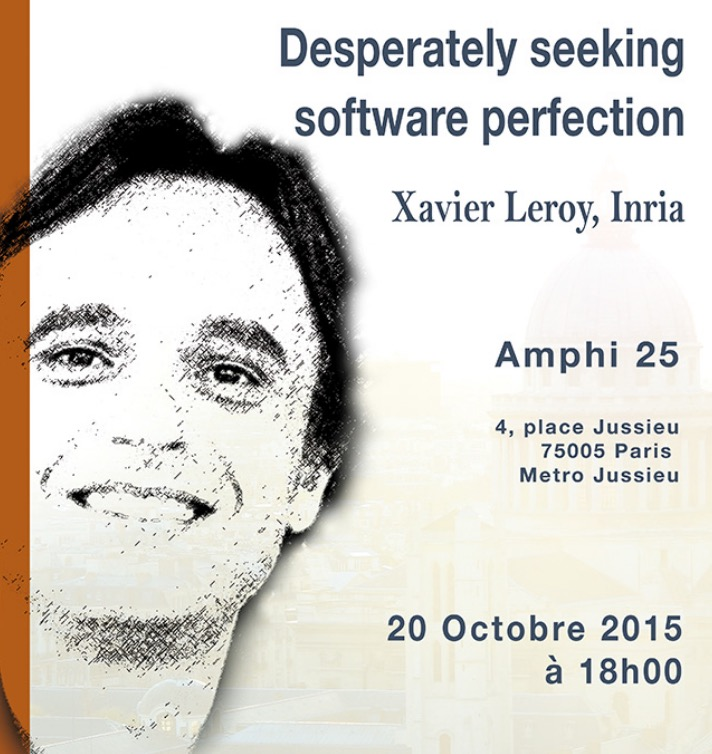
\includegraphics[width=2.25cm]{pics/xavier.jpg}}
\put(85,-50){
\includegraphics[width=3cm]{pics/llvm.png}}
\put(25,-50){
\includegraphics[width=2cm]{pics/gcc.png}}
\end{picture}
\end{frame}


\begin{frame}
  \frametitle{Programming lang. designs and implementations go   wrong.}
 \vspace{-5cm}
\raisebox{0.8cm}{Type Safety of \alt<1-2>{Java {\small{(20 years ago)}}}{Java and
      Scala {\small{(20 years later)}}}}
%  \begin{itemize}
%   \item Run your research {\small{[Klein et al POPL'12]}}
%\\
%{\small{Tested 10 papers -- all of them contained flaws from typos to
%    wrongly stated theorems}}
%\\[1.5em]
%  \item 

% \begin{picture}(0.0,0.0)
% \put(145,-65){
\includegraphics[scale=0.11]{pics/java-type-safe-probably.jpg}}  \pause
% \put(150,-45){
\includegraphics[scale=0.17,angle=45,origin=c]{pics/java-not-type-safe.jpg}}\pause
% \put(180,-95){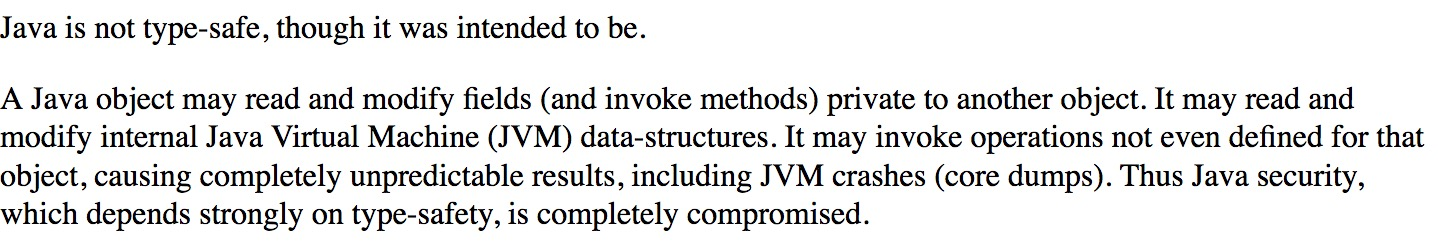
\includegraphics[scale=0.1,angle=45]{pics/java_unsafe.jpg}}
% \put(150,-45){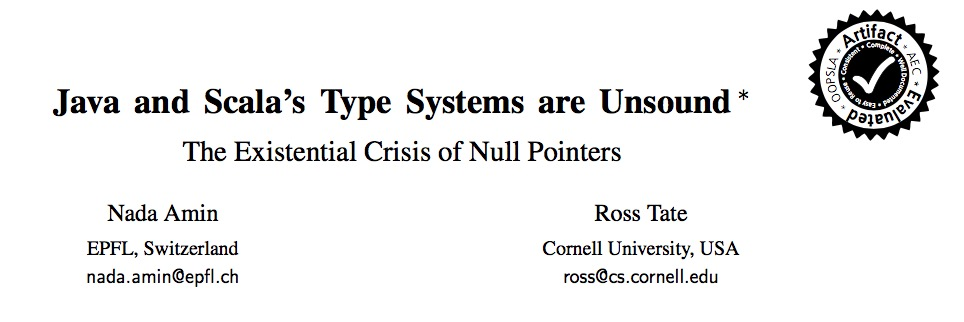
\includegraphics[scale=0.17,angle=-45,origin=c]{pics/Java+Scala-unsound.jpg}}\pause
% \put(137,-55){
\includegraphics[scale=0.1,angle=45]{pics/dot-sound.jpg}}
% \end{picture}

\hspace{1cm}\begin{picture}(0.0,0.0)
\put(25,-145){
\includegraphics[scale=0.17]{pics/java-type-safe-probably.jpg}}  \pause
\put(5,-105){
\includegraphics[scale=0.27,angle=45,origin=c]{pics/java-not-type-safe.jpg}}
\put(45,-205){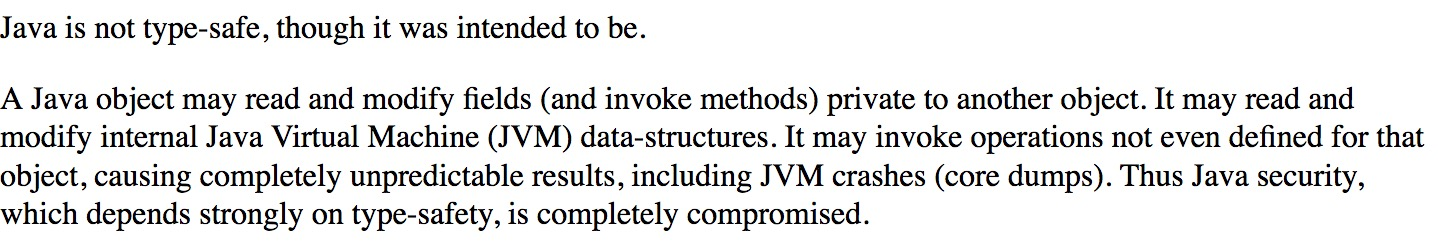
\includegraphics[scale=0.20,angle=45]{pics/java_unsafe.jpg}}\pause
\put(10,-145){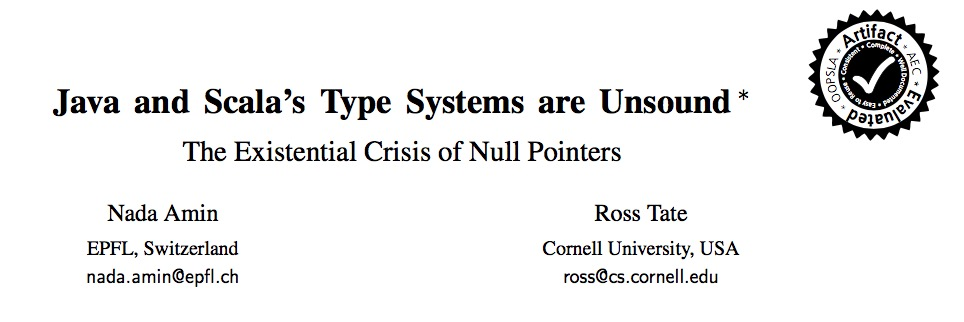
\includegraphics[scale=0.24,angle=-35,origin=c]{pics/Java+Scala-unsound.jpg}}\pause
\put(18,-197){
\includegraphics[scale=0.18,angle=45]{pics/dot-sound.jpg}}
\end{picture}

\end{frame}


\begin{frame}
  \frametitle{The problem}
  \vspace{-3cm}
Correct proofs are tricky to write 
\begin{itemize}
\item a lot of overhead \\(on paper and even more so in a proof assistant)
\item challenging to keep track of details
\item hard to understand interaction between different features
\item difficulties increase with size 
\end{itemize}

\end{frame}

\begin{frame}{Proofs: The tip of the iceberg}

 \begin{center}     
 
\includegraphics[width=10cm,height=5cm,clip=true]{pics/eisberg.jpg}
% % \begin{picture}(0,0)(200,-20)
% %        \put(166,212){Beweischritte}
% %        \put(170,200){}
% %        \put(200,90){\rotatebox{15}{Variablen}}
% %        \put(150,140){\rotatebox{-15}{Annahmen}}
% %        \put(260,130){\rotatebox{-10}{Umbenennung von Variablen}}
% %        \put(200,145){\rotatebox{10}{Ersetzung von Variablen}}
% %        \put(170,120){\rotatebox{5}{context}}
% % \end{picture}
 \end{center}

 \begin{small}
   \begin{tabular}{p{11cm}}
 {\textit{
 ``We may think of [the] proof as an iceberg. In the top of it, we find what we
 usually consider the real proof; underwater, the most  of the matter, consisting
 of all mathematical preliminaries a reader must know in order to understand what
 is going on.'' \hfill S. Berardi [1990]
 }    }
   \end{tabular}

 \end{small}


\end{frame}


  \section{POPLMark -- A Look Back ...}

%----------------------------------------------------------------------------
\begin{frame}\frametitle{POPLMark Challenge: Mechanize System F$_<$ [2005]}%-------------------------------------------------


 Spotlight on

 \begin{center}\begin{tabular}{p{10cm}}
 {\small{\emph{``type preservation and soundness, unique decomposition properties of operational semantics, proofs of equivalence between algorithmic and declarative versions of type systems.''}}}
   \end{tabular}
 \end{center}
\begin{itemize}
\item Structural induction proofs (syntactic)
\item Focus on representing and reasoning about structures with binders
\item Easy to be understood; text book description (TAPL)
\item Small (can be mechanized in a couple of hours or days)
\item Explore more systematically different proof environments
\item Explore different encoding techniques for representing bindings
\end{itemize}

\end{frame}

%----------------------------------------------------------------------------
\begin{frame}\frametitle{POPLMark Challenge -- The Good}%-------------------------------------------------
\vspace{-2.5cm}
\begin{minipage}{9cm}
\begin{itemize}
\item[\checkmark] Popularized the use of proof assistants
\item[\checkmark] Many submitted solutions
\item[\checkmark] Good way to learn about a technique
\item[\checkmark] Mechanizing proofs is addictive!
\\[1ex]
\vspace{0.25ex}
\end{itemize}  
\end{minipage}
\begin{picture}(0.0,0.0)
% \put(+205,-75){
\includegraphics[width=2.75cm]{pics/stick-figure-praying.png}}
\put(-35,-55){
\includegraphics[scale=0.45]{pics/stick_figure_dancing.png}}
\end{picture}
% \pause
% The Bad 
% \begin{itemize}
% \item Did we achieve \emph{``a future where the papers in conferences such as POPL and ICFP are routinely accompanied by mechanically checkable proofs of the theorems they claim.''}?\\[0.5em]
% \item Did we get better tool support for mechanizing proofs?
% \vspace{0.25ex}
% \end{itemize}
% \pause
% The Ugly
% \begin{itemize}
% \item[\xmark] Did not inspired the development of new theoretical foundations
% %\item[\xmark] Did we gain a better understanding of the theoretical
% %  foundations of proof environments?  
% \end{itemize}

\end{frame}


%----------------------------------------------------------------------------
\begin{frame}\frametitle{POPLMark Challenge -- The Bad}%-------------------------------------------------
\vspace{-2cm}
\begin{minipage}{9cm}
\begin{itemize}
\item Did we achieve \emph{``a future where the papers in conferences such as POPL and ICFP are routinely accompanied by mechanically checkable proofs of the theorems they claim.''}?\\[0.5em]
\item Did we get better tool support for mechanizing proofs?
\vspace{0.25ex}
\end{itemize}  
\end{minipage}
%\begin{minipage}{3cm}  
\begin{picture}(0.0,0.0)
 \put(+1,-45){
\includegraphics[width=2.75cm]{pics/stick_figure_thinking-confused.jpg}}
\end{picture}
%\end{minipage}
\end{frame}

%----------------------------------------------------------------------------
\begin{frame}\frametitle{POPLMark Challenge -- The Ugly}%-------------------------------------------------
\vspace{-3cm}
  \begin{minipage}{9cm}
\begin{itemize}
\item[\xmark] Did not identify bugs or flaws in existing systems
\item[\xmark] Did not inspired the development of new theoretical
  foundations
\item[\xmark] Did not push existing systems to their limit
\\[0.5em]
\begin{tabular}{p{7.5cm}}
  \emph{   ``Type soundness results are two a penny.''}\\\quad \hfill Andrew Pitts
\end{tabular}



% \item[\xmark] 
%\item[\xmark] Did we gain a better understanding of the theoretical
%  foundations of proof environments?  
\end{itemize}    
  \end{minipage}
\begin{picture}(0.0,0.0)
 \put(+15,-55){
\includegraphics[width=1.75cm]{pics/head-scratch-VC-num.jpg}}
\end{picture}


\end{frame}


% \begin{frame}\frametitle{} % [standout]
%  \begin{tabular}{p{10cm}}
% \Large \textbf{Beyond the POPLMark Challenge}\\[1em]    
% \color{orange}\hline\\[0.5em]
%   \begin{quote}
% ``The POPLMark Challenge is not meant to be exhaustive: other aspect
% [...] that are interesting [...] to name a few:  
% % other aspects of programming language theory raise formalization difficulties that are interestingly
% % different from the problems we have proposed —- to name a few: more complex
% % binding constructs such as mutually recursive definitions,
% ... \emphFact{logical relations proofs}, coinductive simulation argument,...'' [Aydemir et. al. 2005]
%   \end{quote}
%   \end{tabular}
% \end{frame}



% \section{Proof assistants allow us to mechanize formal systems and proofs.}

% \begin{frame}
%   \frametitle{The Good and the Bad}
  
% The Good:
%   \begin{itemize}
%   \item We don't need to do everything manually
%   \item The system checks whether we got it right
%   \item It's addictive!
%   \end{itemize}

% The Bad:
% \begin{itemize}
% \item A lot of overhead involved (up to 70\%)
% \item Do we still understand the proof?
% \item Do we still understand what we proved?
% \end{itemize}

% \end{frame}




% %----------------------------------------------------------------------------
% \begin{frame}\frametitle{Before 2005: A Brief Incomplete History}%-------------------------------------------------
% % A brief incomplete history of mechanizing meta-theory
% \begin{itemize}
% \item Isabelle [1986], Coq[1989], Alf/Agda~1 [1990 -- 2007], Lego [1995/98], Elf/Twelf[1993/1998], $\ldots$
% \item Case studies: Type Soundness, Church Rosser, Cut-elimination, Compilation, $\ldots$
% \item Focus on reasoning about formal systems by structural induction; modelling variable bindings; assumptions; etc.
% \item Canonical example: Type soundness
% \item Some normalization proofs:
%   \begin{itemize}
%   \item Altenkirch, SN for System F in Lego [TLCA 1993]
%   \item Barras/Werner, SN for CoC in Coq [1997]
%   \item C. Coquand, NbE for $\lambda\sigma$ in ALFA [1999]
%   \item Berghofer, WN for STL in Isabelle [TYPES 2004]
%   \item Abel, WN/SN for STL in Twelf [LFM 2004]
%   \end{itemize}
% \end{itemize}


% \end{frame}

% \section{POPLMark Challenge!}



  \section{Beyond the POPLMark Challenge!
%\begin{picture}(0.0,0.0) 
 %\put(0,0){klklk}  
 %\end{picture}
}

\begin{frame}
  \frametitle{Beyond the POPLMark Challenge}

  \begin{quote}
``The
POPLMark
Challenge is not meant to be exhaustive: other aspects of programming language theory raise formalization difficulties that are interestingly
different from the problems we have proposed —- to name a few: more complex
binding constructs such as mutually recursive definitions,
{\color{orange}{logical relations proofs}}, coinductive simulation arguments, undecidability results, and linear handling of
type environments.'' [Aydemir et. al. 2005]
  \end{quote}


\end{frame}


% \begin{frame}\frametitle{Orbi: Benchmarks for reasoning with binders }%-------------------------------------------------

% Equivalence of algorithmic and declarative equality on normal lambda-terms

% \begin{itemize}
% \item[\checkmark] Highlighted issues surrounding binders and contexts \\(subsumption, context relations)
% \item[\checkmark] Lead to automated support for contexts in Abella [LFMTP'15?]
% \item[\checkmark] Lead to a deeper understanding of the challenges
%   when reasoning with contexts
% \item[\checkmark] Simple, easy to replicate
% \item[\checkmark] Good base line for testing systems
% \vspace{1.5ex}
% %\pause
% \item[---] Narrow focus; narrow impact
% \end{itemize}

% \end{frame}

\section{POPLMark Reloaded -- \newline Goals and Target Audience}
\begin{frame}\frametitle{User community including students and PL researchers:}%-------------------------------------------------
\vspace{-3cm}


  \begin{itemize}
  \item Teach logical relations proofs a modern way 
  \item A good way to learn a useful and wide-spread proof technique
  \item Deeper understanding of the mechanics behind the technique
  \item Understand the trade-offs in choosing a particular proof
    environment when tackling such a proof
  \item Be able to grow the development to rich type theories \\
(ultimate goal: normalization of dependently typed systems)
%  \item Understand how the technique scales
  \end{itemize}





\end{frame}


\begin{frame}\frametitle{Framework developers:}%-------------------------------------------------
\vspace{-3cm}
\begin{itemize}
\item Highlight features that are ideally suited for built-in support
\item Highlight current shortcomings (theoretical and practical) in existing proof environments
\item Benchmark for evaluating and comparing systems
\item Signpost to advertise a given system
\item Stimulate research on foundations of proof environments
\end{itemize}




\end{frame}

% \begin{frame}\frametitle{POPLMark Reloaded: Goals and Audience}%-------------------------------------------------

% Benchmark problems that

% \begin{itemize}
% \item Push the state of the art in the area and outline new areas of research
% \item Compare systems and mechanized proofs qualitatively
% \item Understand what infrastructural parts should be generically supported and factored
% \item Find bugs in existing proof assistants
% % \item Realistic Example
% \item Highlight theoretical limitations of existing proof environments
% \item Highlight practical limitations of existing proof environments
% \end{itemize}

% \end{frame}

\section{POPLMark Reloaded: \newline\protect\color{orange}{Strong normalization for
  the simply-typed lambda-calculus with typed-reductions using
  Kripke-style logical relations} }
%----------------------------------------------------------------------------

\begin{frame}
  \frametitle{Simply Typed $\lambda$-Calculus with Type-Directed
    Reductions}

Simply Typed $\lambda$-calculus:
  
\[
\begin{array}{llcl}
\mbox{Terms}  & M,N & \bnfas & x \mid \lambda x{:A}. M \mid M\;N \\
\mbox{Types} & A, B & \bnfas & \base \mid A \arrow B
\end{array}
\]

\pause 
Type-directed reductions [Goguen'95]:
\[
\begin{array}{c}
\infer[\beta]{\Gamma \vdash (\lambda x{:}A.M)~N  \red [N/x]M : B }
    {\Gamma \vdash \lambda x{:}A.M : A \arrow B & \Gamma \vdash  N : A}
\qquad
%\infer[\eta]{\Gamma \vdash M \red \lambda x{:}A.M~x : A \arrow B}{
% M \not= \lambda y{:}A.M'}
\\[1em]
\infer{\Gamma \vdash M\,N \red M'\,N : B}{\Gamma \vdash M \red M' : A \arrow B & \Gamma \vdash N : A} 
\qquad
\infer{\Gamma \vdash M\,N \red M\,N' : B}{\Gamma \vdash M : A \arrow B & \Gamma \vdash N \red N' : A} 
\\[1em]
\infer{\Gamma \vdash \lambda x{:}A.M \red \lambda x{:}A.M' : A \arrow B}{\Gamma, x{:}A \vdash M \red M' : B}
\end{array}
\]


\end{frame}

\begin{frame}\frametitle{Why Type-directed Reductions?}%-------------------------------------------------


  \begin{itemize}
  \item Allows us to give a concise presentation of the important
    issues that arise.
\item Typed operational semantics simplifies the study of its
  meta-theory.
\item Widely applicable in studying subtyping, type-preserving
  compilation, etc.
\item Types are necessary if we want to allow $\eta$-expansion or
  $\textsf{unit}$ types. 


\[
  \begin{array}{l}
\infer{\Gamma \vdash M \red () : \textsf{unit}}{M \not = ()}  \quad
\infer{\Gamma \vdash M \red \lambda x{:}A.M~x : A \arrow B}{M \not= \lambda y{:}A.M'}
  \end{array}
\]



  \end{itemize}

\end{frame}


\begin{frame}{Setting the Stage: How to define strong normalization?}

Often defined as an accessibility relation:

\[
\infer[]{\csn \Gamma M}{\forall M'.~\Gamma\vdash M\Steps M' \Longrightarrow \csn \Gamma {M'}}
\]
\vspace{1ex}
% \begin{itemize}
% \item Reason about reduction sequences and about positions of terms
% \end{itemize}

\begin{quote}
``the reduct analysis becomes increasingly annoying in normalization
proofs for more and more complex systems.'' \hfill Joachimski and
Matthes  
\end{quote}


\begin{quote}

\end{quote}
\end{frame}

\begin{frame}{A modular approach to strongly normalizing terms}

Alternative approach ({\small{F. van Raamsdonk and P. Severi [1995] and R. Matthes and F. Joachimski [AML 2003]}})
  \begin{itemize}
  \item Inductive characterization of normal forms ($\sn \Gamma M$)
  \item Normalization proof is by induction on normal forms and
type expressions
  \item Leads to modular proofs -- on paper and in mechanizations
%  \item Show: $\csn \Gamma M$ iff $\Gamma \vdash M \in \SN$.
  \end{itemize}

  \begin{quote}
``the new proofs are essentially simpler than already existing ones.''
\hfill F. van Raamsdonk  and P. Severi 
  \end{quote}

\end{frame}

\begin{frame}{Inductive definition of well-typed strongly normalizing terms}
\[
\begin{array}{c}
\multicolumn{1}{l}{\mbox{Neutral terms}} \\[1em]
\ianc{x{:}A \in \Gamma}{\Gamma \vdash x \in \SNe}{} \qquad  
\ibnc{\Gamma \vdash R \in \SNe}{\Gamma \vdash M \in \SN}{\Gamma \vdash R\,M \in \SNe}{} 
\\[1em]
\multicolumn{1}{l}{\mbox{Normal terms}} \\[1em]
\ianc{\Gamma \vdash R \in \SNe}{\Gamma \vdash R \in \SN}{} \qquad 
\ianc{\Gamma, x{:}A \vdash M \in \SN}{\Gamma \vdash \lambda x{:}A.M \in \SN}{} \qquad
\ibnc{\Gamma \vdash M \redSN M'}{\Gamma \vdash M' \in \SN}{\Gamma \vdash M \in \SN}{} 
\\[1em]
\multicolumn{1}{l}{\mbox{Strong head reduction}} \\[1em]
\ianc{\Gamma \vdash N \in \SN}{\Gamma \vdash (\lambda x.M)\;N \redSN [N/x]M}{} \qquad
\ianc{\Gamma \vdash R \redSN R'}{\Gamma \vdash R\,M \redSN R'\,M}{}
\end{array}
\]

\end{frame}

\section{Challenge 1: Equivalence between accessibility and inductive
  definition of strongly normalizing terms:\newline \newline $\csn \Gamma M$ iff $\Gamma \vdash M \in \SN$.}


\begin{frame}
  \frametitle{Challenges in the proof}
  \begin{itemize}
  \item Richer induction principles needed than just structural  induction based on sub-derivations
  \item Model and work with well-scoped and well-typed terms 
  \item Basic infrastructure
    \begin{itemize}
    \item[-] Weakening and Strengthening of type-directed reductions
    \item[-] Weakening and Exchange strongly normalizing terms ($\csn \Gamma  M$)
    \end{itemize}

  \item Reason about different shapes of terms (neutral, reded in head
    position, etc.)
  \end{itemize}
\end{frame}


\begin{frame}{Strong normalization using logical relations}

%  \begin{center}
% \textbf{Reducibility must be defined on well-typed open terms!}
%   \end{center}
%\vspace{1ex}


\pause
% \alt<2>{
\begin{definition}
 [Reducibility Candidates: $\rcs \Gamma M B$]
\mbox{}
\begin{tabular}{l@{~}c@{~}lll}
  $\Gamma \vdash M$ & $\in$ & $\R_B$ & iff & $\Gamma\vdash M\hastype B$
                                          and $\sn \Gamma M$\\
  $\Gamma \vdash M$ & $\in$ & $\R_{T\arrow S}$ & iff &
$ \Gamma\vdash M\hastype {T\arrow S}$ and  \\
  & & & & for all $N,\Delta$ such that
  $\Gamma \leq_\rho \Delta$,  \\
  & & & & ~~~~~~if $\rcs \Delta N {T}$ then
  $\rcs \Delta {([\rho]M) \app N} {S}$.

\end{tabular}
% \begin{itemize}
% \item $\rcs \Gamma M B$ iff $\Gamma\vdash M\hastype B$ and $\sn \Gamma M$
% \item $\rcs \Gamma M {T\arrow S}$ iff
%   $ \Gamma\vdash M\hastype {T\arrow S}$ and for all $N,\Delta$ such that
%   $\Gamma \leq_\rho \Delta$, if $\rcs \Delta N {T}$ then
%   $\rcs \Delta {([\rho]M) \app N} {S}$.
% \end{itemize}
\end{definition}
\vspace{1ex}
\begin{itemize}
\item Contexts arise naturally when we want to state properties about
  well-typed terms and we want to be precise.
\item They are necessary! 
\item The definition scales to dependently typed setting and stating
  properties about type-directed equivalence of lambda-terms.
% type directed reductions
\end{itemize}
\pause
\vspace{1ex}
\alt<3>{\centering \textit{Do we really need the weakening substitution
  $\rho$?}}
{\centering \textit {Do we really need to model terms in a ``local'' context and
  use Kripke-style context extensions?}}
\pause
% }{}

\end{frame}


\section{Challenge 2: Strong normalization  for simply typed
  $\lambda$-calculus \newline \newline
Main fundamental lemma: \newline If $\Gamma \vdash M : A$ and $\Gamma \leq_\rho
\Gamma'$ then $\Gamma' \vdash [\rho]M \in \R_A$. 
}


\begin{frame}
  \frametitle{Challenges in the proof}
\begin{itemize}
  \item Stratified definitions for reducibility candidates (not
    strictly positive!)
  \item Model and work with well-scoped and well-typed terms 
% (comparison between different approaches 
% well-scoped de Bruijn, libraries, contextual types, nominal, 
  \item Basic infrastructure
%    \begin{itemize}
%    \item[-] Weakening and Strengthening of type-directed reductions
%    \item[-] Weakening and Exchange strongly normalizing terms (
% $\csn \Gamma  M$)
Renaming, Anti-renaming, Substitution properties for
      strongly normalizing terms 
%    \end{itemize}
\end{itemize}
%  \item Comparison and trade-offs when modelling well-scoped and
%    well-typed terms
%  \item Good way to gain a deeper understanding of logical relations proofs\\
% $\Longrightarrow$ extension to products, sums, recursion, $\ldots$
\end{frame}



\section{Towards solving the challenge problems}

\begin{frame}
  \frametitle{On the way}
  
  \begin{itemize}
  \item Coq mechanization using Autosubst
\\ -- add pictures of people involved

  \item Abella\\
-- add pictures of people involved

  \item Agda using well-scoped de Bruijn indices
\\ -- add pictures of people involved

\item \beluga
  \end{itemize}
\end{frame}


%----------------------------------------------------------------------------
\begin{frame}[fragile]\frametitle {\beluga: Programming and Proof Environment}
%-------------------------------------------------



\begin{center}     

\includegraphics[width=10cm,height=5cm, clip=true]{pics/eisberg.jpg}\\
\begin{scriptsize}
\begin{picture}(0,0)(200,60)
       \put(185,165){\dRed{Main Proof}}
%       \put(185,155){Beweis}
       \put(190,103){\rotatebox{15}{Eigenvariables}}
       \put(180,130){\rotatebox{-5}{Hypothesis}}
       \put(242,120){\rotatebox{-5}{\mygreen{Context}}}
       \put(230,127){\rotatebox{5}{Variables}}
       \put(170,140){\rotatebox{0}{Renaming}}
       \put(202,90){\rotatebox{25}{\mygreen{Derivation Tree}}}
       \put(180,115){\rotatebox{5}{\mygreen{Substitution}}}
       \put(220,140){\rotatebox{5}{Scope}}
       \put(250,140){\rotatebox{-5}{Binding}}
       \put(68,120){\mygreen{Contextual }}
       \put(68,110){Logical Framework LF}
%       \put(68,110){\mygreen{[TOCL'08,POPL'08,LFMTP'13,...]}}
%        \put(68,180){\dRed{Functional}}
       \put(68,184){\dRed{Functional Programs with}}
       \put(68,174){\dRed{Indexed (Co)data Types}}
%       \put(68,164){\dRed{[POPL'08,POPL'12,}}
%       \put(68,154){\dRed{POPL'13,ICFP'16]}}
\end{picture}  
\end{scriptsize}
\end{center}
\vspace{-1cm}


% \beluga: Abh{\"a}ngig getypte Programmiersprache und Beweiseumgebung
\begin{small}
\begin{itemize}
\item Below the surface: \footnotesize{Support for key concepts based on Contextual
  LF}
{\footnotesize{[TOCL'08,POPL'08,LFMTP'13, ESOP'17, $\ldots$]}}
\item Above the surface: \footnotesize{(Co)Inductive Proofs
    \\\hspace{2cm}~~as (Co)Recursive Programs
  using (Co)pattern Matching} \\% with built-in index language of  Contextual LF objects\\
{\footnotesize{[POPL'08,IJCAR'10, POPL'12,POPL'13,CADE'15,ICFP'16, $\ldots$]}}
\end{itemize} 
\end{small}


\end{frame}


\begin{frame}
  \frametitle{A Quick Guided Tour}
  
Demo

\end{frame}



\begin{frame}\frametitle{A confession ...}
  
What we've done in Beluga so far
\begin{itemize}
\item SN proof with inductive definition 
\item Set up scales to sums and products
\item Built-in support for simultaneous substitutions leads to compact proofs
\end{itemize}

Still to do ...


A confession 

Thanks, Aliya.

\end{frame}


\begin{frame}
  \frametitle{Lessons learned -- The Good}
Elegant.
  \begin{itemize}
  \item HOAS is great!
  \item Built-in support for simultaneous substitutions and renamings
    is great!
  \item Take advantage of dependent types to model intrinsically typed
    terms, typed-reductions, typed $\SN$, etc.
  \item Modular, scales
  \item Compact
  \end{itemize}
\end{frame}

\begin{frame}
  \frametitle{Lessons learned -- The Bad and Ugly}
  \begin{itemize}
  \item How to pattern matching on renamings $[\rho]M$?
  \item Interactive Mode to develop proofs needs work
  \item Termination checker not powerful enough
  \item 
  \end{itemize}

Confession: we are missing implementation or anti-renaming lemmas ...
\end{frame}



\begin{frame}
  \frametitle{Extensions}
  \begin{itemize}
  \item Unit Type 

\[
  \begin{array}{l}
\infer{\Gamma \vdash M \red () : \textsf{unit}}{M \not = ()}  \quad
% \infer{\Gamma \vdash M \red \lambda x{:}A.M~x : A \arrow B}{M \not= \lambda y{:}A.M'}
  \end{array}
\]

  \item Disjoint Sums\\
    (requires closure)

  \item Recursion (G{\"o}del's system T)

  \end{itemize}

\end{frame}



% \begin{frame}\frametitle{Question 2}%-------------------------------------------------
% \vspace{4em}
% \begin{center}
% \LARGE\textbf
% {Why pick strong normalization for simply-typed lambda-calculus using
% Kripke-style
% logical relations?}
% \end{center}

% \pause
% In particular:
% \begin{enumerate}
% \item We can prove SN without (Kripke-style) logical relations and we've already done it.
% % \item
% \end{enumerate}

% \end{frame}

\section{Isn't proving strong normalization in a proof assistant an old hat?}

\begin{frame}\frametitle{Witness 1: Lego [Altenkirch'93]}

$\ldots$ ``following Girard's Proofs and Types''
\\[1em]
Characteristic Features:
  \begin{itemize}
    \item Terms are not well-scoped or well-typed
    \item Candidate relation is untyped and does not enforce
      well-scoped terms
$\Longrightarrow$ does not scale to typed-directed evaluation or equivalence\\
$\Longrightarrow$ maybe better techniques to modularize and structure proof
  \end{itemize}

\end{frame}



\begin{frame}\frametitle{Witness 2: Abella, ATS/HOAS}\relax%-------------------------------------------------
% \pause
$\ldots$ ``following Girard's Proofs and Types''
\pause

\begin{itemize}
% \item Lego [T. Altenkirch'93]: Untyped candidate relation
% - terms are not well-scoped
% - types are are well-scoped
% - Candidate relation is untyped; works on not well-scoped terms;
%   that's why you don't need Kripke-style
%
\item Strictly speaking:% \emph{SN for simply-typed $\lambda$-calculus plus constants.}
\begin{center}
\begin{tabular}{p{10cm}}
\emph{SN for simply-typed $\lambda$-calculus plus one constant.}
\end{tabular}
\end{center}

\item Adding a constant significantly simplifies the proof
\item Reducibility of terms only defined on closed terms
\\[1ex]
\item Strictly speaking:
\begin{center}
\begin{tabular}{p{10cm}}
\emph{Show that SN for simply-typed $\lambda$-calculus plus one
  constant implies also SN for open simply-typed $\lambda$-terms}
\end{tabular}
\end{center}
\end{itemize}

\end{frame}


\begin{frame}
  \frametitle{More Witnesses $\ldots$}

  \begin{itemize}
  \item Berghofer : Program extraction from a proof of weak
    normalization using Isabelle [2004]
\\
$\Longrightarrow$ Uses de Bruijn encoding (not well-scoped or
well-typed)\\
% $\Longrightarrow$ Uses de Bruijn encoding (not well-scoped or well-typed)\\
$\Longrightarrow$ ``Compact'' mechanization (800 lines)
\\[1em]
\pause
\item Berger et al. [TLCA'93]: Extraction of a normalization by
  evaluation using strong evaluation in Minlog\\
$\Longrightarrow$ Uses well-scoped de Bruijn encoding \\% (not
                                % well-scoped or well-typed)
$\Longrightarrow$ Domain theoretic semantics
\\[1em]
\pause
\item Doczkal, Schwinghammer [LFMTP'09]:
Mechanization of Strong Normalization Proof for Moggi’s Computational
Metalanguage in Isabelle/Nominal\\
$\Longrightarrow$ Use of nominals avoids Kripke-style formulation
\end{itemize}
\end{frame}


\section{Beyond strong normalization ...}


\begin{frame}
  \frametitle{Additional Challenge Problems}
  \begin{itemize}
  \item Adding $\eta$-expansion

  \item Type-directed algorithmic equality\\
(done in Beluga)

  \item Weak normalization \\
  (good starting point)

  \item Normalization of System F \\
   (excellent suggestion -- currently beyond what Beluga can do)
  \end{itemize}

\end{frame}



% \begin{frame}{Why Kripke-style?}

%   \begin{itemize}
%   \item Kripke-style extensions cannot be avoided when we attempt to
%     prove properties about type-directed evaluation
% \\
% {\small{(see for example mechanizations of Crary's proof of
%     completenes of algorithmic equality for LF)}}
% \\[1em]
%   \item We want to keep the benchmark problem simple, but it should
%     exhibit features that allow us to scale systems to more complex problems.
%   \end{itemize}


% \end{frame}

\begin{frame}
  \frametitle{Evaluation Criteria}
  

\end{frame}


\begin{frame}{A Call for Action}
  \begin{itemize}
  \item Be part of formulating and tackling the challenge
%  \item Help us prepare a tutorial on strong normalization using
%    Kripke-style logical relations
% states clearly the problem, can be read and then implemented more or
% less straightforwardly
  \item Choose your favorite proof assistant and complete the
    challenge
%   \item Be part of analyzing mechanizations\\[1em]~~
  \end{itemize}

%   \begin{center}
% \Large
% Last but not least: Propose a different challenge!     
%   \end{center}




\end{frame}




  \section{Let's get started...\pause talk to me for the challenge
    problem set up \newline \protect \color{orange}Thank you!}

\end{document}


%%% Local Variables:
%%% mode: latex
%%% TeX-master: t
%%% End:
